\documentclass[11pt]{beamer}
\usepackage[utf8]{inputenc}
\usepackage[T1]{fontenc}

\usepackage[backend=bibtex,style=authoryear]{biblatex}
\addbibresource{brownbags.bib}

%% End of citations additions

%\usetheme{AnnArbor}
%\usetheme{Antibes}
%\usetheme{Berkeley}
%\usetheme{Berlin}
%\usetheme{boxes}
%\usetheme{Darmstadt}
%\usetheme{default}
%\usetheme{Frankfurt}
%\usetheme{Ilmenau}
%\usetheme{JuanLesPins}
\usetheme{Luebeck}
%\usetheme{Malmoe}
%\usetheme{Montpellier}
%\usetheme{PaloAlto}
%\usetheme{Rochester}
%\usetheme{Singapore}
%\usetheme{Szeged}
%\hypersetup{
%	colorlinks=true,
%	linkcolor=blue,
%	filecolor=magenta,      
%	urlcolor=cyan,
%}

\setbeamertemplate{footline}
{%
	\leavevmode%
	\hbox{\begin{beamercolorbox}[wd=.2\paperwidth,ht=2.5ex,dp=1.125ex,leftskip=.3cm,rightskip=.3cm plus1fill]{author in head/foot}%
			\usebeamerfont{author in head/foot} \insertframenumber{} / \inserttotalframenumber
		\end{beamercolorbox}%
		\begin{beamercolorbox}[wd=.3\paperwidth,ht=2.5ex,dp=1.125ex,leftskip=.3cm plus1fill,rightskip=.3cm]{author in head/foot}%
			\usebeamerfont{author in head/foot}\insertshortauthor
		\end{beamercolorbox}%
		\begin{beamercolorbox}[wd=.5\paperwidth,ht=2.5ex,dp=1.125ex,leftskip=.3cm,rightskip=.3cm plus1fil]{title in head/foot}%
			\usebeamerfont{title in head/foot}\insertshorttitle
	\end{beamercolorbox}}%
	\vskip0pt%
}
\setbeamertemplate{headline}{}

\begin{document}
	\author{Gary R Seamans}
	\title{Regression Modeling}
	\subtitle{R Brown Bag Series \#4}
	%\logo{\scalebox{0.035}{
\includegraphics{R_logo.png}}}
	\institute{The MITRE Corporation}
	%\date{}
	%\subject{}
	%\setbeamercovered{transparent}
	%\setbeamertemplate{navigation symbols}{}
	\begin{frame}[plain]
		\maketitle
    \end{frame}

\begin{frame}{
	\begin{minipage}[t]{0.55\textwidth}
		Agenda
	\end{minipage}
	\hfill
	\begin{minipage}[t]{0.35\textwidth}
		\flushright
		\scalebox{0.035}{
\includegraphics{R_logo.png}}
	\end{minipage}
}{}
%% ==================== Content ===========================%%
\begin{center}
	\begin{itemize}
		\item Overview
		\item Demonstrations
		\item Questions
	\end{itemize}
\end{center}
\end{frame}

%% Overview ===================
\begin{frame}{
	\begin{minipage}[t]{0.55\textwidth}
		Overview
	\end{minipage}
	\hfill
	\begin{minipage}[t]{0.35\textwidth}
		\flushright
		\scalebox{0.035}{
\includegraphics{R_logo.png}}
	\end{minipage}
}{}
%% ==================== Content ===========================%%
\textit{Statistical modeling, regression analysis is a set of statistical processes for estimating the relationships among variables.}\parencite{regressionWiki} Wikipedia is not an authoritative source, but this is a reasonable operating definition of regression modeling.

\vspace{0.5cm}

\cite{harrell2001ordinal} is, with well over 8k citations, a very authoritative source for regression modeling. A less expensive (read free) alternative is \parencite{harrell2013regression} which is a version of the book Dr. Harrell uses to teach regression modeling at Vanderbilt. A copy of the free version is included in the download material.  

\end{frame}

%% Overview Continued ===================
\begin{frame}{
	\begin{minipage}[t]{0.55\textwidth}
		Overview contd.
	\end{minipage}
	\hfill
	\begin{minipage}[t]{0.35\textwidth}
		\flushright
		\scalebox{0.035}{
\includegraphics{R_logo.png}}
	\end{minipage}
}{}
%% ==================== Content ===========================%%
What kinds of regression are there? \href{https://www.r-bloggers.com/15-types-of-regression-you-should-know/?utm\_source=feedburner\&utm\_medium=email\&utm\_campaign=Feed\%3A+RBloggers+\%28R+bloggers\%29}{\textcolor{blue}{\underline{This article}}} from \href{https://www.r-bloggers.com/}{\textcolor{blue}{\underline{R-bloggers}}} describes 15 different types of regression. Which one to use?
\begin{columns}
	\begin{column}[t]{0.45\textwidth}
		\begin{itemize}
			\item Linear Regression
			\item Polynomial Regression
			\item Logistic Regression
			\item Quantile Regression
			\item Ridge Regression
			\item Lasso Regression
			\item Elastic Regression
			\item Principal Component Regression
		\end{itemize}
		\end{column}
	\begin{column}[t]{0.45\textwidth}
			\begin{itemize}
				\item Partial Least Square Retgression
				\item Support Vector Regression
				\item Ordinal Regression
				\item Poisson Regression
				\item Negative Binomial Regression
				\item Quasi-Poisson Regression
				\item Cox Regression
			\end{itemize}
	\end{column}
\end{columns}

\end{frame}


%% Fitting ===================
\begin{frame}{
\begin{minipage}[t]{0.55\textwidth}
	Fitting
\end{minipage}
\hfill
\begin{minipage}[t]{0.35\textwidth}
	\flushright
	\scalebox{0.035}{
\includegraphics{R_logo.png}}
\end{minipage}
}{}
%% ==================== Content ===========================%%
Two of the pitfalls to avoid are:
\begin{itemize}
	\item Overfitting
	\item Underfitting
\end{itemize}
\begin{center}
	\scalebox{0.09}{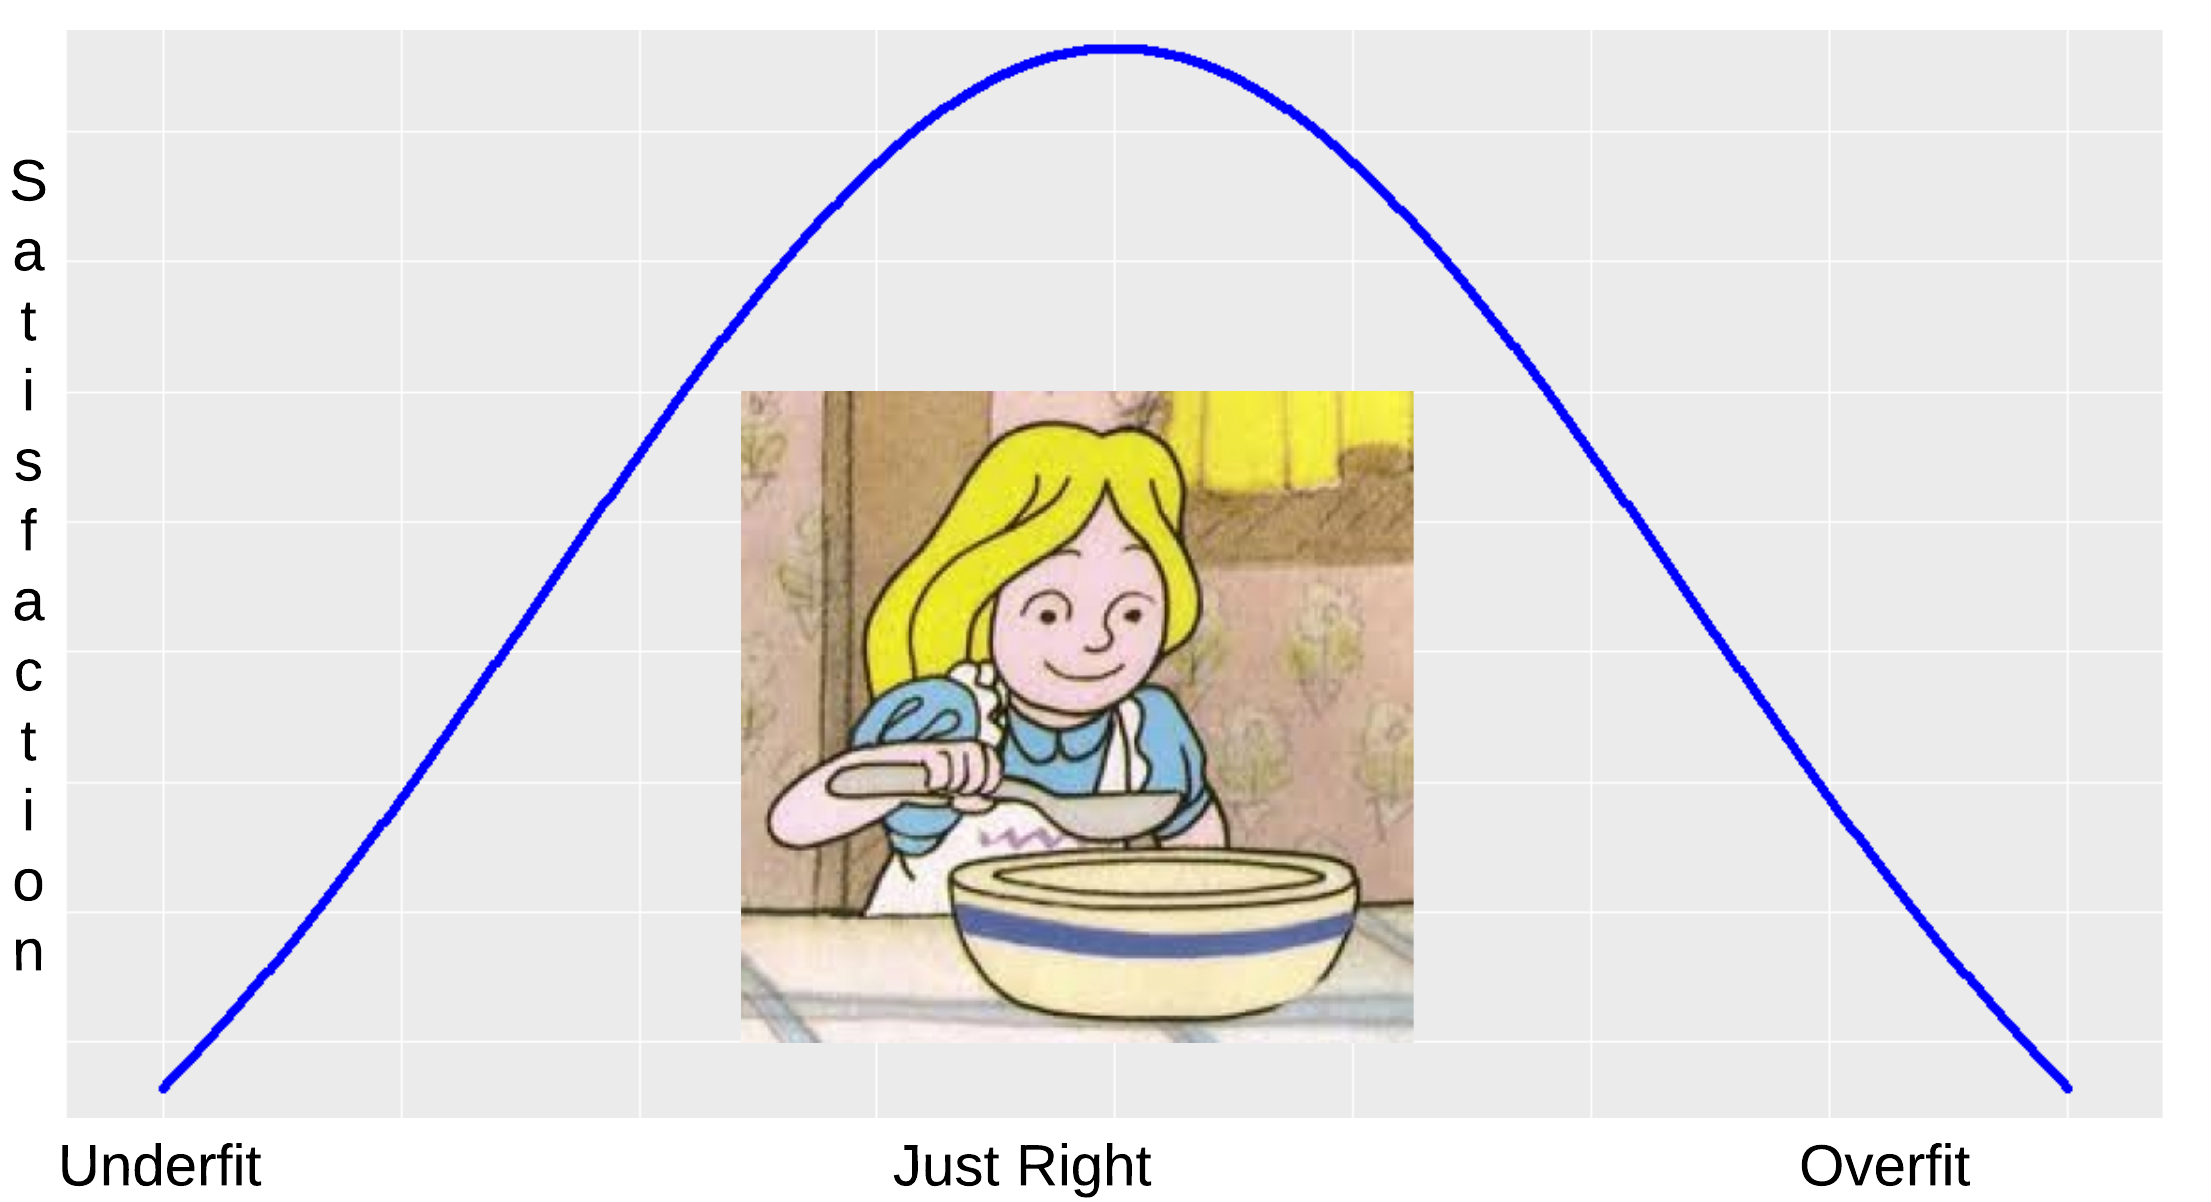
\includegraphics{goldilocks.png}}
\end{center}

\end{frame}

%% Fitting ===================
\begin{frame}{
	\begin{minipage}[t]{0.55\textwidth}
		Fitting Continued
	\end{minipage}
	\hfill
	\begin{minipage}[t]{0.35\textwidth}
		\flushright
		\scalebox{0.035}{
\includegraphics{R_logo.png}}
	\end{minipage}
}{}
%% ==================== Content ===========================%%
Fitting graphic from the R-bloggers post\parencite{fitting_graphic}.

\begin{center}
	\scalebox{0.40}{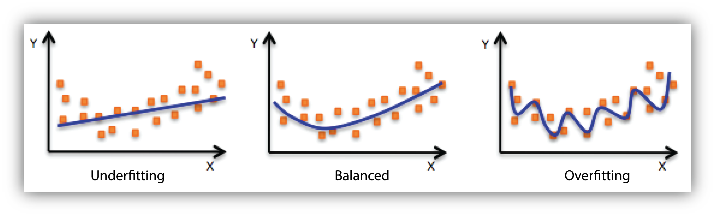
\includegraphics{Fitting.png}}
\end{center}

\end{frame}

%% additional terms ===================
\begin{frame}{
	\begin{minipage}[t]{0.55\textwidth}
		Additional Terms
	\end{minipage}
	\hfill
	\begin{minipage}[t]{0.35\textwidth}
		\flushright
		\scalebox{0.035}{
\includegraphics{R_logo.png}}
	\end{minipage}
}{}
%% ==================== Content ===========================%%
Additional Regression Terminology.

\begin{itemize}
	\item Outliers - can unduly influence the results
	\item Multicollinearity - highly correlated independent variables
	\item Heteroscedasticity - when a dependent variable's value is not equal across values of an independent variable
\end{itemize}


\end{frame}

%% Galtons Data  ===================
\begin{frame}{
	\begin{minipage}[t]{0.55\textwidth}
		Galton's Data
	\end{minipage}
	\hfill
	\begin{minipage}[t]{0.35\textwidth}
		\flushright
		\scalebox{0.035}{
\includegraphics{R_logo.png}}
	\end{minipage}
}{}
%% ==================== Content ===========================%%
In this example we'll look at Galton's data. Sir Francis Galton was an 18th century statistician, among other things, and his data on the relative heights of children and their parents is still relevant today. 

\vspace{0.5cm}

There are a number of ways to get the Galton dataset, one is to download the R package \textbf{UsingR}. Typing \textbf{data()} in an R console will list all of the available datasets. You'll probably be surprised at how many come with the default installation. 

\vspace{0.5cm}

To load the Galton data you would use \textbf{data(galton)}, more correctly you would create a \textit{promise} that the Galton data will be loaded the first time it is referenced. Typing \textbf{summary(galton)} will cause the Galton data to be loaded and display a set of summary statistics.
 
\begin{center}

\end{center}
\end{frame}



%% Credit Card Default ===================
\begin{frame}{
	\begin{minipage}[t]{0.55\textwidth}
		Credit Card Default
	\end{minipage}
	\hfill
	\begin{minipage}[t]{0.35\textwidth}
		\flushright
		\scalebox{0.035}{
\includegraphics{R_logo.png}}
	\end{minipage}
}{}
%% ==================== Content ===========================%%
Credit card default is a big problem for banks. This example of multivariate regression shows how you might go about predicting who will default.
\begin{center}
	
\end{center}
\end{frame}

\usebackgroundtemplate{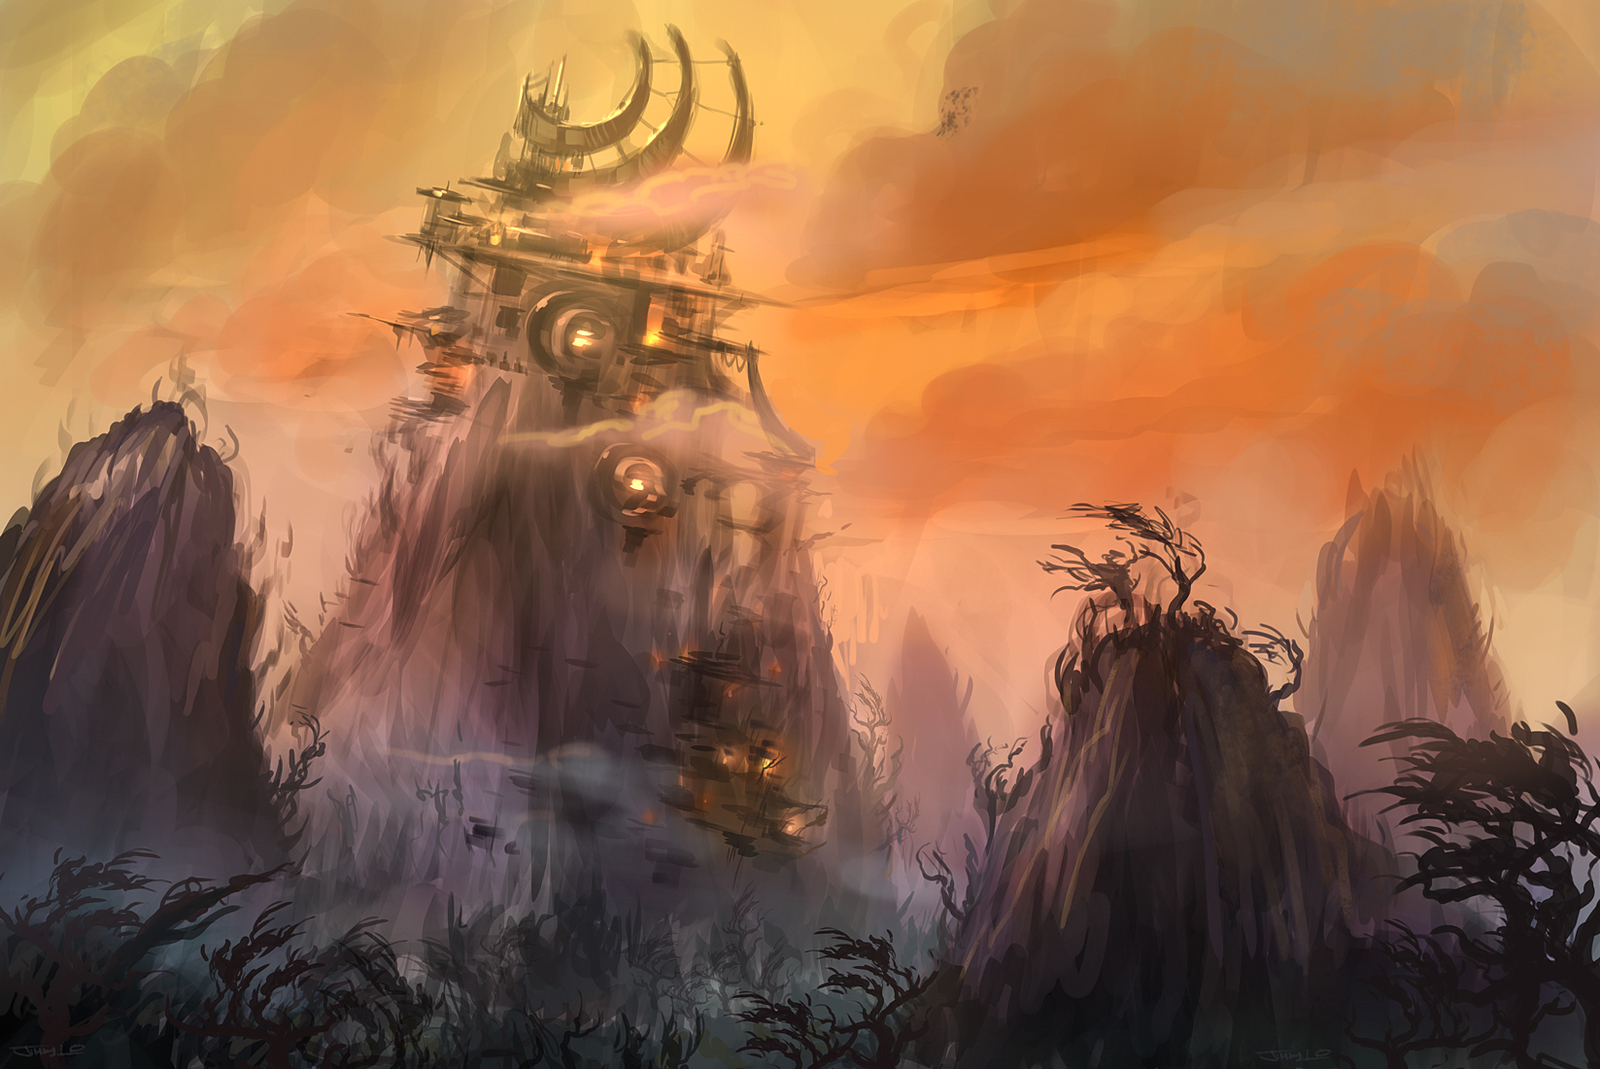
\includegraphics[width=\paperwidth, height=\paperheight]{wow_art1.jpg}}
%% Questions ===================
\begin{frame}{
	\begin{minipage}[t]{0.55\textwidth}
		Questions
	\end{minipage}
	\hfill
	\begin{minipage}[t]{0.35\textwidth}
		\flushright
		\scalebox{0.035}{
\includegraphics{R_logo.png}}
	\end{minipage}
}{}
%% ==================== Content ===========================%%
\begin{center}
	
\end{center}
\end{frame}

\usebackgroundtemplate{}

%%===================== Citations =================================%%
\appendix
\begin{frame}[allowframebreaks]{References}{}
\footnotesize
\printbibliography

\end{frame}
\end{document}